% Basic setup
\documentclass[12pt,a4paper]{article} % Defines the document type as an article with 12pt font size on A4 paper.
\usepackage{siunitx}
\sisetup{separate-uncertainty=true,exponent-product = \cdot,
} \usepackage{amsmath}
% Importing packages
\usepackage[english]{babel} % Sets the document language to English, adjusting hyphenation and language-specific typographic rules.
\usepackage[lmargin=2.5cm,rmargin=2.5cm,tmargin=2cm,bmargin=2cm]{geometry} % Sets custom page margins: left/right 2.5cm, top 2cm, bottom 2cm.

\usepackage{hyperref}    % Enables hyperlinks for references, URLs, and citations.
\usepackage{xcolor}      % Provides tools for defining and using colors.
\usepackage{graphicx}    % Allows inclusion of images and graphics.
\usepackage{caption}     % Customizes captions for figures and tables.
\usepackage{subcaption}  % Supports subfigures and subcaptions within figures.
\usepackage{minted}      % Enables syntax highlighting for code listings.
\usepackage[T1]{fontenc} % Ensures proper font encoding, important for correct character rendering. Don't touch this.
\usepackage{setspace}    % Provides control over line spacing.
\usepackage{csquotes}    % Improves handling of quotations.
\usepackage{longtable,booktabs,array} % Packages for advanced table formatting.
\usepackage[
  backend=biber,
  style=apa,  
]{biblatex}  % Manages citations and bibliography with APA style.

\definecolor{LightGray}{gray}{0.9}  % Defines a custom color 'LightGray' with 90% gray, used for the code block background.
\hypersetup{                        % Configures hyperlink colors and behavior.
  colorlinks=true,                  % Enable colored links instead of boxes.
  linkcolor={blue},                 % Sets link color to blue.
  filecolor={maroon},               % Sets file link color to maroon.
  citecolor={blue},                 % Sets citation link color to blue.
  urlcolor={blue}}                  % Sets URL link color to blue.

\providecommand{\tightlist}{        
  \setlength{\itemsep}{0pt}\setlength{\parskip}{0pt}}

\addbibresource{assets/bib-template.bib} % Adds the bibliography file.

\title{Lab Report}        % Sets the document title.
\makeatletter
\providecommand{\subtitle}[1]{%     % Custom command to add a subtitle.
  \apptocmd{\@title}{\par {\large #1 \par}}{}{}
}
\makeatother
\subtitle{Spectroscopy}  % Sets the document subtitle.
\author{Alexandra Pernisova}         % Sets the author's name.
\date{2024-08-01}                   % Sets the document date.

% From this point, the preamble ends and the actual content of the document starts.
\begin{document}
\renewcommand{\arraystretch}{1.3}
\pagenumbering{gobble} % Stops counting the pages from this point until changed again.
\maketitle

\begin{center}
    \vfill
    \begin{figure}
        \centering
        \begin{subfigure}{.3\textwidth}
          \centering
          \includegraphics[width=.8\linewidth]{./assets/uni-basel-logo-en.png}
        \end{subfigure}%
        \begin{subfigure}{.3\textwidth}
          \centering
          \includegraphics[width=.8\linewidth]{./assets/dhlab-logo-black.png}
        \end{subfigure}
        \end{figure}
        \setcounter{figure}{0}
        
    University of Basel\\
    Digital Humanities Lab\\
    Switzerland
\end{center}
\newpage
\renewcommand*\contentsname{Table of Contents} % This controls the title of your table of contents.
{
\hypersetup{linkcolor=}
\setcounter{tocdepth}{5} % Sets the maximum sublevel to be displayed within the table of contents.
\tableofcontents
}
\newpage
\pagenumbering{arabic}\setstretch{1.5} % Overwrites the previous command, pages are counted as normal from this point.

\section{The Single Photon Source}
\subsection{Introduction}
    In the following experiments a single photon source will be used. The single photon source used is a type of an SPDC source. The first experiment stands to take preliminary measurements.
\subsection{Methods and Materials}
    The source used is a \textit{quED qutools} SPDC source. A non-linear crystal is used to convert some of the incoming laser-beam photons to photon pairs or other down converted variations of multiple photons. The source is therefore in terms of single-photon pairs a heralded source, meaning that the measurement of a photon in one arm heralds a photon in the other. 

    The pump laser is a diode laser of \qty{405}{\nano\meter} operated at \qty{50}{\milli\ampere}. Inside the SPDC encasing (see \ref{diagram:setup}) an arrangement of phase-matchers, BBO-crystals converts some of the pump photons into photon-pairs. Inserting a half-wave plate (see \ref{diagram:setup}) rotates the polarisation to produce an entangled photon-pair.

    Throughout the experiment the control arm acts as a herald for the photon in the signal arm. Either arm couples into an optical fiber that connects to the \textit{qutools} single photon detector. 
    
    The detector measures photon counts at each arm - Single0 $S0$ at control arm and Single1 $S1$ at signal arm. The coincidence rate of the two arms $C01$ is measured in a time-window of \qty{40}{\nano\second}, also known as the gate time $\Delta t_g$. Due to the window duraiton an accidental count measure $N_{acc}$ can be calculated $N_{acc} = S0 \cdot S1 \cdot \Delta t_g$. Furthermore the detector sometimes counts a photon when there is none, which can be measured as the darkcount $N_{dc}$ with laser turned off.

    The setup process of the arangement as shown in diagramm \ref{d1} made use of the alignment laser to roughly align the setup and maximizing the count numbers on the detector by fine-tuning the mirrors.
\subsection{Results}
The preliminary measurements can be seen in Table \ref{tab:preliminary} where the uncertainties are calculated as the Shot noise on the basis of the discrete nature of photon-counting. The fluctuations on the detector readings were taken into consideration and observed to be well-represented by the shot noise.
\begin{table}[h]
\begin{tabular}{l|r|r}
               & \multicolumn{1}{l}{\text{Preliminary Counts (counts/s)}} & \multicolumn{1}{l}{\text{Dark Counts (counts/s)}}
               \\ \hline
Single 0  $S0$     & \qty{138260 \pm 370}{}                                                  & \qty{4000 \pm 100}{}                                            \\
Single 1     $S1$  & \qty{126220 \pm 360}{}                                                  & \qty{7400 \pm 200}{}                                            \\
Coincidence 01 $C01$ & \qty{7948 \pm 89}{}                                                    & \qty{0 \pm 1}{}                                             
\end{tabular}
\caption{Measurement of maximally aligned counts (Preliminary Counts) and Dark Counts }
\label{tab:preliminary}
\end{table}
The calculation of accidental counts $N_A$ and error propagation yields (see Eq. \ref{eq:accidentalcounts}):
\begin{align*}
    N_A = \qty{689 \pm 3}{counts\per\second}
\end{align*}
\subsection{Discussion}
The calculated accidental count rate is around 10 times smaller than the coincidence, the coincidence counts are significantly higher than the accidental counts.

Throughout the experiments the setup was re-aligned a couple of times. The dark counts stayed consistent while the preliminary counts varied up to 30\%. 


\section{Polarization of light}
\subsection{Introduction}
In this experiment the Stokes' vector of an entangled photon pair will be measured. Specifically the different Stokes's parameters will be measured through the intensities of different light polarizations (H...horizontal, V...vertical, D...diagonal, A...antidiagonal.)
\begin{align}
        S_0 = I_0 &= I_H + I_V = I_D + I_A = I_R + I_L
        \label{eq:stokesparams}
\end{align}
\begin{align}
    S_1 &= \frac{I_H - I_V}{I_0} & S_2 &= \frac{I_D + I_A}{I_0} & S_3 &= \frac{I_R + I_L}{I_0}
    \label{eq:stokesparams}
\end{align}
The zeroth Stoke's parameter describes the total intensity of the light. The 3 other parameters can be visually represented on a Stoke's sphere (see fig \ref{fig:stokekes}), which with their help fully describes a polarization state. Following, any state lying on the sphere's surface is a pure state, and any state inside of it a mixed state.
%stokes sphere


\subsection{Methods and Materials}
The source with the HWP (see figure \ref{fig:setup}) produces an entangled pair of photons in a state $H_1 H_2 + V_1 + V_2$. The setup is firstly engaged without QWP and both signal and control polarizers in. The polarizer in each arm are callibrated at a time. The polarizer is rotated while its corresponding single counts are measured and fitted according to Malus' Law (see Eq. \ref{eq:malus}). The $\theta_0$ which maximizes the single counts is identified with the horizontal axis of the polarizer. Subsequently, the QWP in the signal arm is callibrated the same way$\xi_0$ retrieved. The displayed uncertainties are given by the fluctuations seen on the device (around 2\%) if not smaller than the shot noise, the degree uncertainty is given by the resolution \qty{\pm2}{\deg}.
%When the plane of polarization is parallel to one of the axes, a waveplate has no effect on linearly polarized light, but when incident linearly polarized light is 45° to the quarter-wave plate, the one of the horizontal/vertical components of the polarized light receives the π/2 phase shift 

The individual Stokes' parameters are determined by measuring the intensity of each of the polarization states H, V, D, A, R, L (see eq. \ref{eq:stokesparams}). An appropriate polarizer and QWP arrangement is chosen for each state and the intensity measured through coincidence counts. 

\subsection{Results}
The callibration of the polarizer in the control arm (see fig. \ref{fig:control_cos_squared}) yielded the angle of the horizonal axis with respect to lab frame $\theta_0$. The uncertainty is given by the device precision since the standard deviation of fit parameters is smaller.
\begin{align*}
    \theta_{C0} &= \qty{120 \pm 2}{\degree}
\end{align*}
\begin{figure}[h]
    \centering
    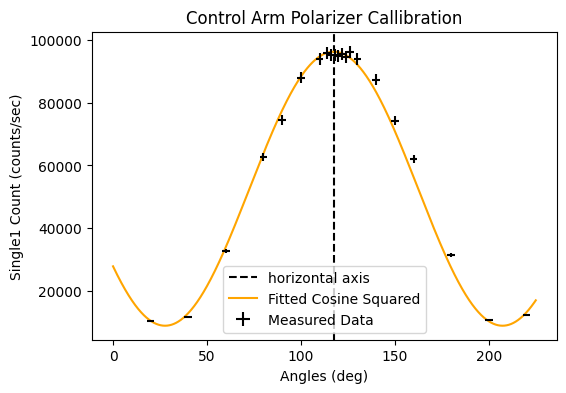
\includegraphics[width=0.8\textwidth]{cntrolarm_fit.png}
    \caption{Control Arm Polarizer Fit for determining the angle of the horizontal axis $\theta_C0$}
    \label{fig:control_cos_squared}
\end{figure}
Similarly, the callibration of the polarizer in signal arm was done over the Coincidence01 and Signal Single0 counts.
\begin{align*}
    \theta_{S0} &= \qty{29 \pm 2}{\deg}
\end{align*}
\begin{figure}[h]
    \centering
    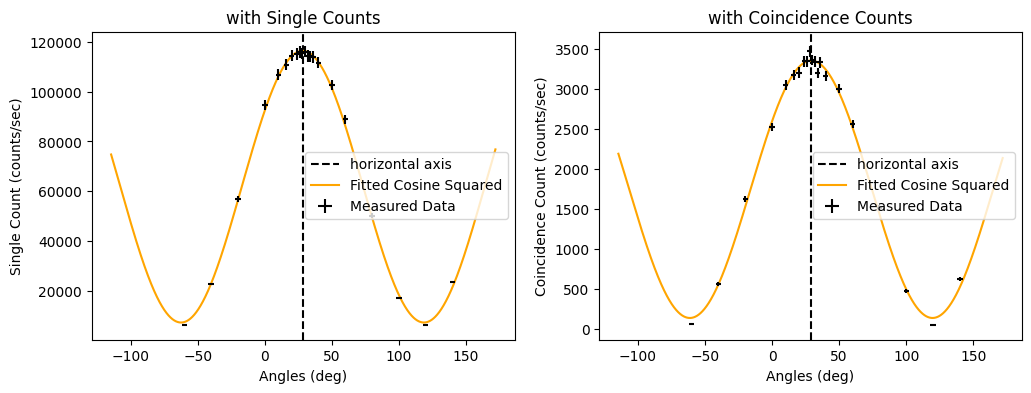
\includegraphics[width=1\textwidth]{signal_arm.png}
    \caption{Signal Arm Polarizer Fits for determining the angle of the horizontal axis $\theta_S0$}
    \label{fig:control_cos_squared}
\end{figure}
The QWP was callibrated to its horizontal (or vertical) angle.
The angle of maximal transmission identified with the horizontal axis $\xi_0$ was determined with uncertainties from the parameter's standard deviation.
\begin{align*}
    \xi_0 = \qty{87 \pm 8}{\deg}
\end{align*}
\begin{figure}[h]
    \centering
    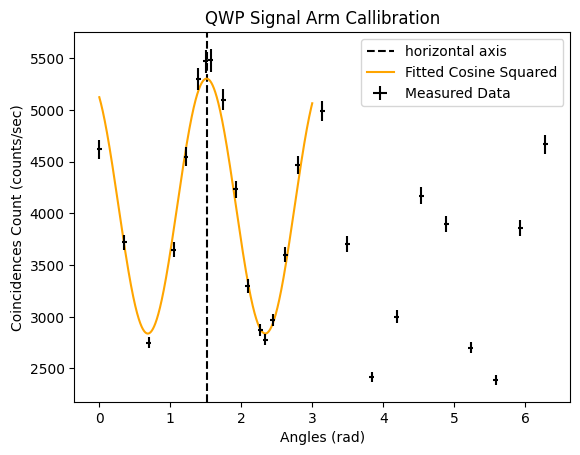
\includegraphics[width=0.6\textwidth]{qwp_callibration.png}
    \caption{QWP Callibration for determining the angle of the horizontal axis $\xi_0$}
    \label{fig:signalpolarizer fit}
\end{figure}
The measurement of coincidence counts for different control polarizer alignments and the resulting stokes parameters are shown in table \ref{tab:stokesparam}. The uncertainties are propagated from the shot noise.
\begin{table}[]
\begin{tabular}{|l|r|r|r|r|}
\hline
  & \multicolumn{1}{l|}{S1} & \multicolumn{1}{l|}{S2} & \multicolumn{1}{l|}{S3} & \multicolumn{1}{l|}{V} \\ \hline
H & $0.826\pm0.019$  &$ -0.159\pm0.031$   &$ -0.078\pm 0.030 $  & $0.842\pm0.027  $  \\ \hline
V & $-0.9325 \pm 0.0087$   & $-0.060 \pm 0.026$ & $0.058 \pm 0.025$  & $0.934 \pm 0.012 $ \\ \hline
D &$ -0.464 \pm 0.024$ & $0.736 \pm 0.019$ & $0.377 \pm 0.025$  & $0.870 \pm 0.036$  \\ \hline
A & $-0.322 \pm 0.026$ & $-0.807 \pm 0.016$  & $-0.338 \pm 0.025$ & $0.870 \pm  0.032$  \\ \hline
\end{tabular}
\caption{Stokes Parameters of the }
\label{tab:stokesparams}
\end{table}

\subsection{Discussion}
We can see that the Bell state is uneven, since the Stokes parameters for the no-polarizer case return uneven cases. As expected the Stokes parameters for the entangled states that get measured in the control arm to a certain polarization, show this polarization in the signal arm as well. This demonstrates the entanglment. 

Otherwise the propagated uncertainties are not big enough to include the expected results, which would be 1-0 pairs for the axis of polarization and 50-50 for other polarization pair. This is assumed to also come from the imperfect state of the photon pair, which might not only include the entangled Bell state, but also other mixed states, which contribute to the uneven measuremetn results.

\section{The Michelson Interferometer}
\subsection{Introduction}
This experiments uses a Michelson Morley Interferometer setup to investigate the interference of the source's photon pairs.
A Michelson Interferometer splits an incoming wave at a beam splitter. The two arms are then mirrored and interfere at at the beam splitter once again given that they are coherent. An interference pattern can be observed in dependence of the phase shift due to optical path length difference of the arms and demonstrates wave-like nature of the observed interferee.

\subsection{Methods and Materials}
For this experiment a Michelson Morley \textit{qutools} Module is connected to the signal arm via the coupled fiber. The module can be seen in fig. \ref{}. The optical path length difference can be measured via a movable glass wedge with varying thickness (see eq. \ref{eq:wedge}). Here the index of refraction in glass for a wavelenght of $\qty{810}{\nano\meter}$ (of the down converted photon pair) is used.
\begin{align}
    \Delta d &= blueblue
\label{eq:wedge}
\end{align}
The inserted module makes for an additional path length in comparison with the control arm, therefore an extra loop of fibre is inserted in this arm. For further considerations, the gate window duration is converted to 'allowed' difference in optical path of the two arms that will still register as a coincidence, which is $\approx \qty{12}{\meter}$. The coincidences are assumed to be unaffected by the difference in the path difference between the two arms.

The control arm acts as a herald against which the signal arm's possible interference pattern is going to be measured. The coincidence count between the two $C_{01}$ is measured against small shifts of the glass wedge. The wedge is pushed by a micrometer screw whose precision gives the uncertainty to \qty{\pm 20}{\micro\meter}. The interference pattern is fitted (see eq. \ref{}) and the wavelength as well as the transversal coherence length determined.
%composite fitting fucntion

\subsection{Results}
The coincidence count measurement and the composite fit can be seen in fig. \ref{fig:interferometry fit}. 
\begin{align*}
    \xi_0 = \qty{87 \pm 8}{\deg}
\end{align*}
\begin{figure}[h]
    \centering
    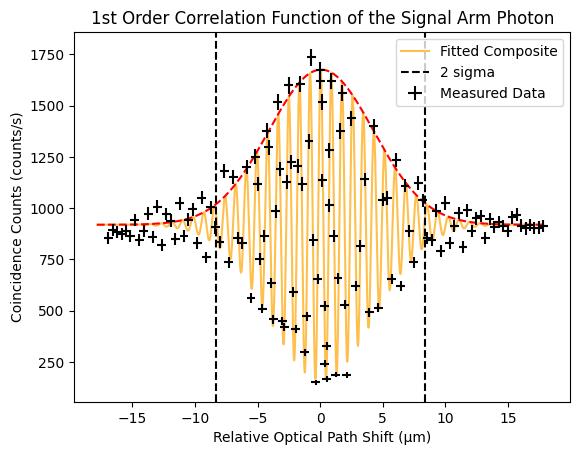
\includegraphics[width=0.6\textwidth]{interferometer.png}
    \caption{The observed interference pattern and its evaluation}
    \label{fig:interferometry fit}
\end{figure}
The coherence length of the photon was determined via a 2 standard deviation spread to each side ($\pm 2\sigma$) (see fig \ref{fig:interferometry fit}), the uncertainty is given by the micrometer precision which is bigger than the fit uncertainty.
\begin{align*}
    L_C &= \qty{16.7 \pm 1.4}{\micro\meter} 
\end{align*}

\subsection{Discussion}
The visible interference pattern shos that the photon exhibits wave-like behaviour. The photon over the 2 arms inside the interferometer interferes with itself. This can be explained by the quantum wave-like nature of photons.

Connecting the interferometer module into the setup and measuring the interference pattern a considerable drop in coincidence counts can be observed. The largest suspected source of loss is the increased instances of fiber-air transitions and the imperfect alignment/coupling.

\section{The Hanbury Brown Twiss Setup}
\subsection{Introduction}
In this experiment a series of measurements on the Hanburry Brown Twiss interferometer will be performed and the second order correlation function of a single photon determined.

The HBT interferometer measured the intensity of the field (or particle in this case) at two different times and their correlation function gives information of longitudinal coherence, also known as the temporal coherence. For a wave a full coherence of 1 is expected at no time separation with a decrease in time. However, for a single classical particle would yield 0 since it can only be at one detector at a time.


\subsection{Methods and Materials}
The setup consists of an HBT module connected to one arm. Inside the module a beamsplitter forks into two outputs which are then connected to the detector. 

At the detector the single counts of all 3 inputs, as well as pair-wise and triple coincidence counts are measured. A series of 10 measurements over 10 second intervals is taken.   

The field intensity formulation of the second order correlation function can be adapted to count measurements over a certain time interval.


\subsection{Results}

\begin{table}[]
\begin{tabular}{l|rrrrrrl}
          & \multicolumn{1}{l}{S0 (herald)} & \multicolumn{1}{l}{S1} & \multicolumn{1}{l}{S2} & \multicolumn{1}{l}{C01} & \multicolumn{1}{l}{C02} & \multicolumn{1}{l}{C012} & C12            \\ \hline
avg       & $\qty{1465300 \pm 1500}{}$ & \qty{307500 \pm 4300 }  & \qty{347600 \pm 5800}{} & \qty{2586 \pm 37}{}   & \qty{2778\pm60}{}  & \qty{2 \pm 1}{} & \textbf{} \\
No Herald & ${20500 \pm 200}$ & ${311480 \pm 770} $& ${351230 \pm 860}$ & ${53 \pm 10}$ & ${21 \pm 4}$ & ${0 \pm 0}$                                & \multicolumn{1}{r}{${331 \pm 31}$}
\end{tabular}
\caption{Counts on the HBT module}
\label{tab:HBT}
\end{table}

%part 2: accidental rate compare
\end{document}